\documentclass[11pt]{article}

% Change "review" to "final" to generate the final (sometimes called camera-ready) version.
% Change to "preprint" to generate a non-anonymous version with page numbers.
\usepackage[review]{acl}

% Standard package includes
\usepackage{times}
\usepackage{latexsym}
\usepackage{booktabs}
% For proper rendering and hyphenation of words containing Latin characters (including in bib files)
\usepackage[T1]{fontenc}
% For Vietnamese characters
% \usepackage[T5]{fontenc}
% See https://www.latex-project.org/help/documentation/encguide.pdf for other character sets

% This assumes your files are encoded as UTF8
\usepackage[utf8]{inputenc}

% This is not strictly necessary, and may be commented out,
% but it will improve the layout of the manuscript,
% and will typically save some space.
\usepackage{microtype}

% This is also not strictly necessary, and may be commented out.
% However, it will improve the aesthetics of text in
% the typewriter font.
\usepackage{inconsolata}

%Including images in your LaTeX document requires adding
%additional package(s)
\usepackage{graphicx}
\usepackage{subcaption}

% If the title and author information does not fit in the area allocated, uncomment the following
%
%\setlength\titlebox{<dim>}
%
% and set <dim> to something 5cm or larger.

\title{Behavior2Value: A Benchmark for Measuring Consumer Values from E-commerce Behaviors}

% Author information can be set in various styles:
% For several authors from the same institution:
% \author{Author 1 \and ... \and Author n \\
%         Address line \\ ... \\ Address line}
% if the names do not fit well on one line use
%         Author 1 \\ {\bf Author 2} \\ ... \\ {\bf Author n} \\
% For authors from different institutions:
% \author{Author 1 \\ Address line \\  ... \\ Address line
%         \And  ... \And
%         Author n \\ Address line \\ ... \\ Address line}
% To start a separate ``row'' of authors use \AND, as in
% \author{Author 1 \\ Address line \\  ... \\ Address line
%         \AND
%         Author 2 \\ Address line \\ ... \\ Address line \And
%         Author 3 \\ Address line \\ ... \\ Address line}

\author{First Author \\
  Affiliation / Address line 1 \\
  Affiliation / Address line 2 \\
  Affiliation / Address line 3 \\
  \texttt{email@domain} \\\And
  Second Author \\
  Affiliation / Address line 1 \\
  Affiliation / Address line 2 \\
  Affiliation / Address line 3 \\
  \texttt{email@domain} \\}

%\author{
%  \textbf{First Author\textsuperscript{1}},
%  \textbf{Second Author\textsuperscript{1,2}},
%  \textbf{Third T. Author\textsuperscript{1}},
%  \textbf{Fourth Author\textsuperscript{1}},
%\\
%  \textbf{Fifth Author\textsuperscript{1,2}},
%  \textbf{Sixth Author\textsuperscript{1}},
%  \textbf{Seventh Author\textsuperscript{1}},
%  \textbf{Eighth Author \textsuperscript{1,2,3,4}},
%\\
%  \textbf{Ninth Author\textsuperscript{1}},
%  \textbf{Tenth Author\textsuperscript{1}},
%  \textbf{Eleventh E. Author\textsuperscript{1,2,3,4,5}},
%  \textbf{Twelfth Author\textsuperscript{1}},
%\\
%  \textbf{Thirteenth Author\textsuperscript{3}},
%  \textbf{Fourteenth F. Author\textsuperscript{2,4}},
%  \textbf{Fifteenth Author\textsuperscript{1}},
%  \textbf{Sixteenth Author\textsuperscript{1}},
%\\
%  \textbf{Seventeenth S. Author\textsuperscript{4,5}},
%  \textbf{Eighteenth Author\textsuperscript{3,4}},
%  \textbf{Nineteenth N. Author\textsuperscript{2,5}},
%  \textbf{Twentieth Author\textsuperscript{1}}
%\\
%\\
%  \textsuperscript{1}Affiliation 1,
%  \textsuperscript{2}Affiliation 2,
%  \textsuperscript{3}Affiliation 3,
%  \textsuperscript{4}Affiliation 4,
%  \textsuperscript{5}Affiliation 5
%\\
%  \small{
%    \textbf{Correspondence:} \href{mailto:email@domain}{email@domain}
%  }
%}

\begin{document}
\maketitle
\begin{abstract}
Personal values provide stable and interpretable signals for understanding user decisions, yet they are rarely observed or annotated in real-world e-commerce recommendation. To address this gap, we introduce the Behavior-to-Value (B2V) task, which aims to identify users’ consumption value orientations from e-commerce behavior trajectories. We construct B2V-Bench, the first large-scale dataset and benchmark for this task. Its construction follows a two-stage methodology: we first develop an e-commerce-specific consumption value taxonomy derived from real-world reviews and aligned with established value theories; we then propose a multi-agent behavioral PVQ framework that enables automated, scalable, and auditable annotation from pre-purchase behaviors. Building on B2V-Bench, we further propose B2V-Model, a Value Verification Tuning (VVT) framework that learns both value label prediction and evidence-based value verification. Experiments show that B2V-Model achieves the best performance among multiple baselines, improving accuracy by xxx.
\end{abstract}

\section{Introduction}
Human values are stable beliefs about desirable goals and principles, guiding how individuals interpret situations and act across contexts~\cite{}. Studying human values is crucial for uncovering the deeper motivational structures underlying behavior, thereby offering a foundational perspective for explaining persistent patterns in human judgment, behavior, and social interaction.

%这一段需要精炼
In e-commerce recommendation, user behaviors are often driven by deeper personal values. Compared with specific interests and short-term preferences, personal values are more abstract and stable, reflecting the ideal states that users seek to attain. Value is important for recommendation because it can explain observed choices and help recommend items that may not match immediate preferences but align with users’ deeper value orientations~\cite{}. However, in real-world e-commerce scenarios, user values are rarely explicitly expressed or annotated. We observe that users’ behavioral processes (browsing, favoriting, and adding items to cart and so on) can reveal their underlying value orientations. For example, extensive review checking may indicate risk aversion, while a preference for official stores may reflect brand trust. Based on this insight, we propose the Behavior-to-Value task, which aims to identify the value orientations manifested in users’ consumption decisions from e-commerce behavior trajectories. This task is valuable for improving the accuracy, interpretability, and generalization ability of recommendation systems.

\begin{figure*}[t]
    \centering    
    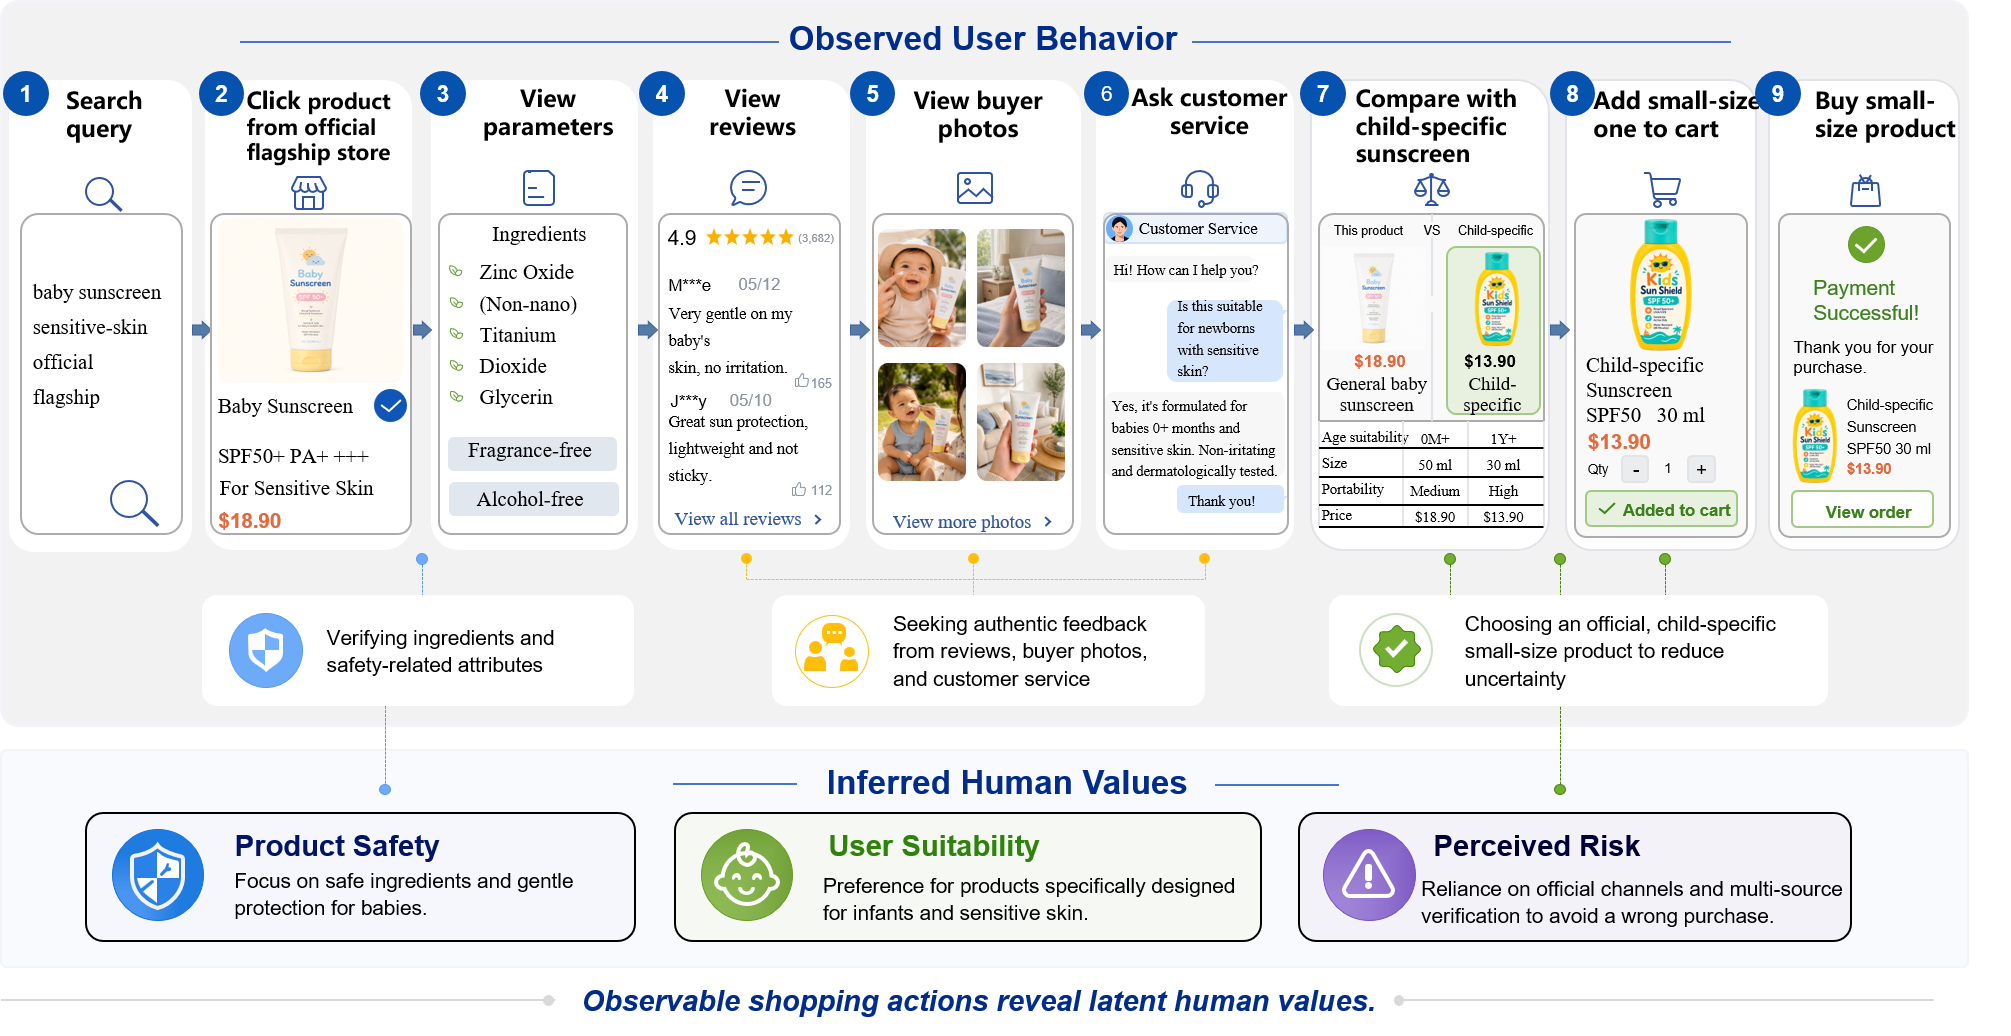
\includegraphics[width=\linewidth, keepaspectratio]{image/teaser3.png}
    \caption{Pseudo-Balancing Vs. True Specialization And Results.
Top: Pseudo-balancing equalizes load but misaligns semantics, causing expert overlap and impeding specialization; true specialization co-routes similar tokens, yielding distinct expertise and less redundancy. Bottom: MAR-MoE augments load-balanced Llama-MoE (baseline MoE) with Memory-Aware Routing, achieving 50\% fewer experts (25\% fewer parameters) without loss and a 35\% increase in specialization.}
      \label{fig:pseudo-balance}
\end{figure*}

%下面这段的(1)和(2)要润色一下表达
However, existing methods are limited for the B2V task. Traditional sequential models mainly learn correlations between user states and item representations to predict future interactions, but they cannot adequately capture the value orientations embedded in product attributes, behavioral actions, and decision contexts. Although LLMs offer stronger semantic understanding, B2V remains challenging for two reasons: (1) existing e-commerce datasets mostly contain coarse-grained interaction logs, such as clicks, favorites, add-to-cart actions, and purchases, lacking fine-grained evidence of how users compare, weigh, and verify alternatives before purchase; (2) value measurement is not a standard classification problem: it requires inferring latent value constructs from indirect and sparse behavioral evidence. Directly mapping behavior sequences to value labels may therefore lead models to learn superficial correlations rather than evidence-supported value judgments.

To address these challenges, we construct B2V-Bench, the first large-scale Behavior-to-Value dataset and benchmark, which contains users’ e-commerce behavior trajectories, such as queries, clicks, and add-to-cart actions, together with their corresponding consumption value labels. The construction of B2V-Bench follows a two-stage methodology. In the first stage, we construct ECVT, an e-commerce-specific consumption value taxonomy. Since existing psychological value theories are often too high-level to capture the fine-grained motivations behind online shopping decisions, we derive value dimensions from large-scale real-world e-commerce reviews, which provide rich and context-specific evidence of users’ consumption concerns, and align them with expert knowledge from classic consumption value scales. In the second stage, we propose a multi-agent behavioral PVQ framework, which transfers the portrait-based measurement logic of the Portrait Value Questionnaire into the analysis of real pre-purchase behavior. This framework preserves the theoretical grounding of established value measurement while enabling automated, scalable, and auditable behavior-based value annotation.

Building on this dataset, we propose B2V-Model, a Value Verification Tuning (VVT) framework for behavior-to-value measurement. Instead of directly learning behavior-to-label mappings, VVT supervises the model with accepted labels, rejected labels, behavioral evidence, counter-evidence, and construct boundary rules. This enables the model to learn both label prediction and evidence-based value verification. As a result, B2V-Model better distinguishes closely related value constructs and produces more faithful, auditable explanations, improving accuracy by xxx.


The main contributions are summarized as follows:
\begin{itemize}
    \item To the best of our knowledge, we are the first to propose the Behavior-to-Value (B2V) task, which identifies users’ value orientations from e-commerce behavior trajectories and offers a new perspective for improving recommendation accuracy, interpretability, and cross-scenario generalization.

    \item We construct B2V-Bench, the first large-scale Behavior-to-Value dataset and benchmark, containing users’ behavior trajectories in real-world e-commerce scenarios with their corresponding consumption value labels. We further develop ECVT, an e-commerce-specific consumption value taxonomy, and an agent-driven behavioral PVQ annotation framework, enabling automated, scalable, and auditable value annotation from behavioral evidence.

    \item We propose B2V-Model, a framework based on Value Verification Tuning for behavior-to-value measurement. It enables the model to learn not only which value label to predict, but also how to assess whether a value inference is sufficiently supported by behavioral evidence. In systematic evaluations across multiple models, B2V-Model achieves the best performance and improves accuracy by xxx.

\end{itemize}




\section{Related Work}



\section{Value Construct}
A prerequisite for constructing a Behavior-to-Value dataset is an e-commerce-specific value taxonomy. Although classic consumption value theories~\cite{} provide foundational accounts of purchase decisions, they predate the rise of online commerce and are too high-level to capture the fine-grained, context-dependent motivations in modern e-commerce. Recent works~\cite{} have explored LLM-based value construction or evaluation, but they mainly focus on general human values rather than consumption values for e-commerce recommendation. 

E-commerce reviews offer a natural data source for grounding the construction of a consumption value taxonomy, as they capture users’ retrospective evaluations of products, services, and shopping experiences in specific consumption contexts. We therefore extract value dimensions from real-world review data and align them with established consumption value scales, resulting in ECVT, the E-commerce Consumption Value Taxonomy.

ECVT aims to derive a fine-grained, interpretable, and theoretically grounded value taxonomy from real e-commerce contexts. Its construction integrates two complementary sources: real user reviews and established consumption value scales. Specifically, we stratify 329,452 reviews from Amazon Reviews 2023 across 33 product categories. As post-purchase evaluations, these reviews directly reflect the value concerns users express about products, services, and shopping experiences. In parallel, we collect 46 established consumption value scales, covering 200 value dimensions and 917 declarative items from major frameworks such as TCV, PERVAL, Holbrook, CPV Meta, CSI, E-S-QUAL, and WebQual. These scales do not directly determine the final taxonomy; instead, they serve as expert priors to guide value cue extraction, ground the discovered dimensions theoretically, and assess framework coverage during validation.

Atomic value cues are extracted from reviews using an LLM agent guided by TCV and priors from 46 established value scales. Each review is decomposed into independent, self-contained evaluative snippets that reflect users’ judgments about price, quality, convenience, service, emotional experience, and related concerns. This process yields about 330K atomic value cues from approximately 330K reviews. These cues are further used to derive candidate value dimensions. Instead of mapping text to a predefined label set, the agent generates a structured candidate dimension for each cue, including its name, definition, decision role, polarity, and TCV affiliation. This design supports open-ended discovery while keeping the outputs organized for subsequent merging and interpretation.

Since the initial candidate pool contains many synonymous, overlapping, and long-tail expressions, dimension merging and cleaning are applied. Highly similar dimensions are first merged through sentence-transformer-based semantic clustering, followed by LLM-based judgments of semantic equivalence and overlap. Low-representativeness singleton noise is removed, and lower-frequency dimensions are mapped to higher-frequency ones when appropriate. Through this process, the raw candidate dimensions are consolidated into 30 final value dimensions and their sub-factors.

%这里讲价值体系的构建

\section{Multi-Agent Annotation Framework}
%名字还要斟酌一下

\begin{figure*}[t]
    \centering    
    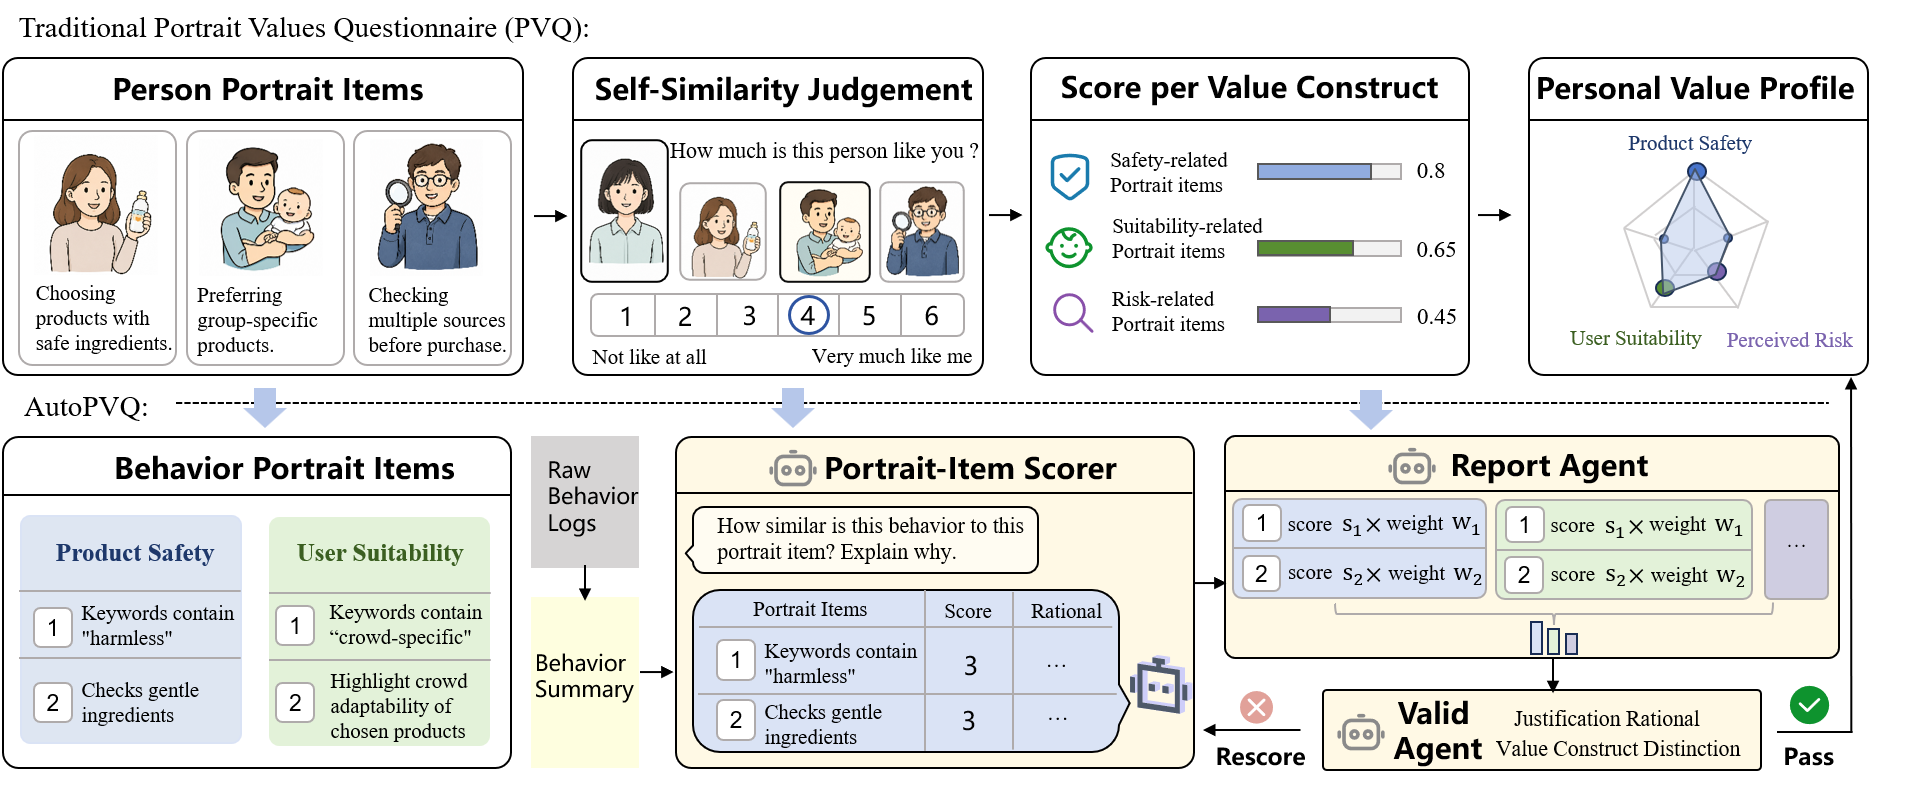
\includegraphics[width=\linewidth, keepaspectratio]{image/annotation1.png}
    \caption{Pseudo-Balancing Vs. True Specialization And Results.
Top: Pseudo-balancing equalizes load but misaligns semantics, causing expert overlap and impeding specialization; true specialization co-routes similar tokens, yielding distinct expertise and less redundancy. Bottom: MAR-MoE augments load-balanced Llama-MoE (baseline MoE) with Memory-Aware Routing, achieving 50\% fewer experts (25\% fewer parameters) without loss and a 35\% increase in specialization.}
      \label{fig:pseudo-balance}
\end{figure*}

How can we measure users’ consumption values from real pre-purchase behaviors? Although traditional self-report value questionnaires~\cite{} offer a mature measurement paradigm, but they are costly, difficult to scale, and poorly suited for dynamic updates. To overcome these limitations, we propose the Multi-Agent Behavioral PVQ Framework, which adapts the portrait-based measurement logic of Portrait Values Questionnaire (PVQ)~\cite{} to behavioral data. 

The key idea of PVQ is to represent each value construct with concrete person portraits and ask respondents to judge how similar each portrait is to themselves. Inspired by this psychometric paradigm, we represent each consumption value as a set of behavioral portrait items that capture its typical manifestations in e-commerce behaviors, and infer the underlying value constructs by matching a user’s pre-purchase behavior against these items. 

To automate this PVQ measurement process, we design a multi-agent system with collaborative specialization and iterative self-correction. Given a summary of a user’s pre-purchase behavior, the system evaluates its match with each value-specific behavioral portrait item, aggregates item-level scores into construct-level value scores, and assigns primary and secondary value labels. By following a well-established value measurement paradigm while enabling automated and scalable annotation, the framework improves both the reliability and practicality of behavior-based value annotation.

\subsection{Value Construct Operationalization Protocol}
Drawing on the measurement logic of value instruments such as PVQ, which represent abstract value constructs through concrete descriptions, we develop the Value Construct Operationalization Protocol (VCOP). VCOP operationalizes abstract consumption values into observable behavioral indicators, providing guidance for counter-evidence verification and construct discrimination, thereby ensuring the reliability and theoretical validity of value annotation.

For each consumption value construct, VCOP specifies five components: the value dimension, its motivational goal, observable behavioral cues as behavioral portrait items, counter-evidence, and rules for distinguishing confusable constructs. Specifically, it defines which behavioral evidence supports a value label, when the evidence is insufficient, which behaviors weaken or reject the label, and which adjacent value constructs require further discrimination.

The construction of VCOP involves two stages: theory-driven initialization and iterative refinement. We first develop an initial version of the protocol based on psychological value scales, e-commerce review data, and consumer psychology literature. Under VCOP, annotators are guided to follow a hierarchical judgment procedure. Rather than directly inferring which values a user holds, they first identify concrete behavioral manifestations in the pre-purchase episode, then interpret the decision strategies reflected by these behaviors, and finally assign consumption value labels according to the mapping rules specified in VCOP. This hierarchical operationalization decomposes an otherwise abstract and subjective value judgment into a series of more concrete and fine-grained decisions, thereby reducing the influence of individual annotators’ personal interpretations and improving the standardization, interpretability, and credibility of the annotations.

We further refine VCOP through multiple rounds of pilot annotation and disagreement analysis. In each round, annotators apply the current version of VCOP to a set of behavior episodes. We then analyze cases involving annotation disagreement, ambiguous evidence, over-inference, and confusion between adjacent value labels. Based on these cases, we revise value definitions, add boundary examples, refine counter-evidence rules, and improve the mapping among behavioral manifestations, decision strategies, and value labels. This iterative process continues until pilot annotation agreement reaches an acceptable level. The finalized VCOP is then used as the theoretical foundation and operational guideline for subsequent large-scale multi-agent value annotation.


\subsection{Multi-agent Annotation System}
Building on the Value Construct Operationalization Protocol (VCOP), we propose a multi-agent framework for behavior-to-value annotation. Inspired by the PVQ-based value measurement process, the framework decomposes annotation into behavioral summarization, profile-item scoring, knowledge augmentation, discriminative verification, feedback refinement, and result aggregation. Each agent performs specialized judgments according to its assigned role, while cross-agent verification and feedback-based refinement jointly form a collaborative reasoning process. Compared with direct label assignment, this design enables automatic iterative correction, thereby reducing potential misclassifications and improving the structure, interpretability, and reliability of the annotation process.

The Behavioral Summary Agent converts raw behavior logs into standardized behavioral descriptions as stable observational input for subsequent value annotation. For behaviors associated with the same purchase goal, it summarizes key actions, such as search, page dwell time, add-to-cart, purchase, and other relevant interactions, while identifying what the user intended to buy, how they compared alternatives, what information they focused on.

The Portrait-Item Scorer matches the behavioral summary against the behavior-profile items defined in VCOP and assigns a support score to each item to assess its alignment with each value construct. Since the value implications of e-commerce behaviors often depend on product attributes, category semantics, store types, and consumption contexts, the scorer leverages the broad semantic knowledge of LLMs to contextualize behavioral evidence. For example, product cues such as “portable” and “installation-free” may indicate the value construct of convenience. Importantly, such semantic knowledge is used only to support the interpretation of observable evidence; the final value judgment remains constrained by VCOP and the behavioral evidence.

Similar to PVQ, the Quality and Report Agent aggregates multiple item-level scores to estimate construct-level support. For each value construct \(v\), let \(I_v\) denote its associated VCOP items. Given the item score \(s_i \in \{0,1,2,3\}\) assigned by the Portrait-Item Scorer, the raw support score is computed as:
\[
\mathrm{RawScore}(v)=\frac{\sum_{i \in I_v} w_i s_i}{\sum_{i \in I_v} w_i},
\]
where \(w_i\) denotes the diagnostic weight of item \(i\). Items aligned with the final purchase choice, observed across multiple decision stages, or defined as strong cues in VCOP receive higher weights.

To capture the relative salience of each value within the episode, the agent applies episode-level centering:
\[
\mathrm{Score}(v)
=
\mathrm{RawScore}(v)
-
\frac{1}{|V|}
\sum_{v' \in V}
\mathrm{RawScore}(v'),
\]
where \(V\) is the set of candidate value constructs.

The agent then assigns the \textbf{primary label} to the highest-scoring construct if it exceeds \(\tau_1\), and assigns a \textbf{secondary label} when another construct exceeds \(\tau_2\) and has independent evidence. If the evidence is weak or the top scores are indistinguishable, the sample is marked as \textbf{uncertain} for human review. The final output includes the labels, a quality score, and an evidence summary.

The Discriminant Agent performs counter-evidence-based verification of the candidate value constructs and support scores produced by the scorer. Based on the distinction rules and counterfactual questions defined in VCOP for closely related constructs, it examines whether a candidate label suffers from construct confusion, insufficient evidence, or conflicts with the observed behavior. For medium- and high-scored candidates, the agent verifies the label using the behavioral summary, supporting evidence, and scoring rationale, and assesses whether it is better supported than alternative interpretations. When potential issues are identified, the Discriminant Agent provides targeted feedback to the scorer, triggering re-scoring and rationale revision. This forms an iterative correction loop of initial judgment, challenge, revision, and re-verification. If a candidate label still fails discriminative verification after multiple rounds, the sample is marked as uncertain and sent for human review, avoiding forced annotation when label boundaries are ambiguous or evidence is insufficient.

\section{Dataset Evaluation and Analysis}
\begin{table*}[t]
\centering
\caption{Statistics of the B2V dataset by TCV dimension for train, validation
and test splits: the number of distinct value constructs, the number of
sessions, the number of behavior-interactions extracted from the session
summary, and the average session length.}
\label{tab:b2v-stats}
\setlength{\tabcolsep}{4pt}
\resizebox{\textwidth}{!}{%
\begin{tabular}{l|c|ccc|ccc|ccc}
\toprule
       &              & \multicolumn{3}{c|}{\textbf{Train}} & \multicolumn{3}{c|}{\textbf{Val}} & \multicolumn{3}{c}{\textbf{Test}} \\
\textbf{TCV Dimension} & \textbf{\#Constructs} & \textbf{\#Sessions} & \textbf{\#Interact.} & \textbf{Avg.\ Len.} & \textbf{\#Sessions} & \textbf{\#Interact.} & \textbf{Avg.\ Len.} & \textbf{\#Sessions} & \textbf{\#Interact.} & \textbf{Avg.\ Len.} \\
\midrule
Functional   & 12 & 3{,}294 & 124{,}154 & 751 & 401 & 15{,}199 & 746 & 405 & 15{,}288 & 757 \\
Emotional    &  4 &   574 &  20{,}954 & 788 &  79 &  2{,}785 & 758 &  83 &  3{,}148 & 798 \\
Social       &  5 &   158 &   5{,}953 & 676 &  16 &    550 & 638 &  14 &    514 & 720 \\
Epistemic    &  4 &    46 &   1{,}623 & 679 &   4 &    121 & 598 &   3 &    118 & 774 \\
Conditional  &  5 &   219 &   7{,}430 & 694 &  33 &  1{,}167 & 699 &  33 &  1{,}181 & 720 \\
\midrule
\textbf{Total} & \textbf{30} & \textbf{4{,}352} & \textbf{162{,}134} & \textbf{748} & \textbf{544} & \textbf{20{,}209} & \textbf{739} & \textbf{544} & \textbf{20{,}428} & \textbf{759} \\
\bottomrule
\end{tabular}%
}
\end{table*}


\begin{figure*}[t]
\centering
\begin{subfigure}{0.32\textwidth}
  \centering
  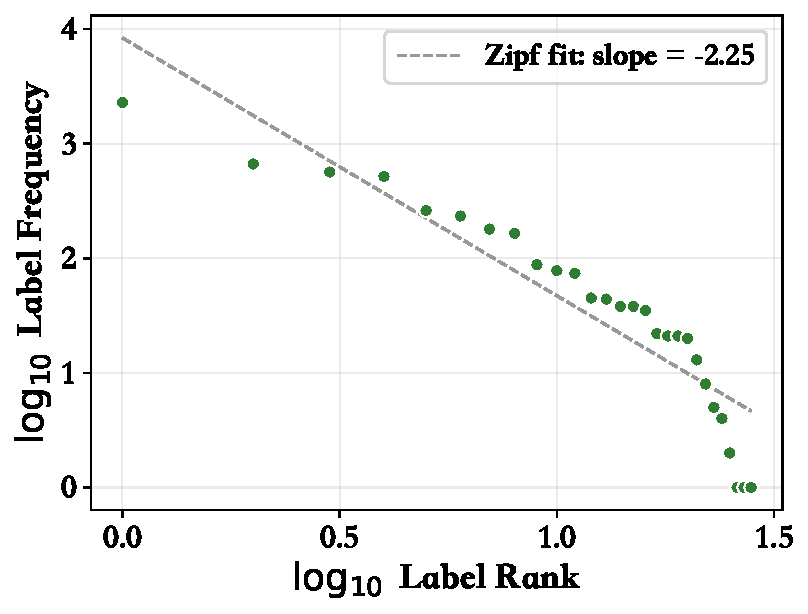
\includegraphics[width=\linewidth]{image/figs/fig1_label_loglog.pdf}
  \caption{Label frequency (Zipf, slope $=-2.25$)}
  \label{fig:b2v:zipf}
\end{subfigure}\hfill
\begin{subfigure}{0.32\textwidth}
  \centering
  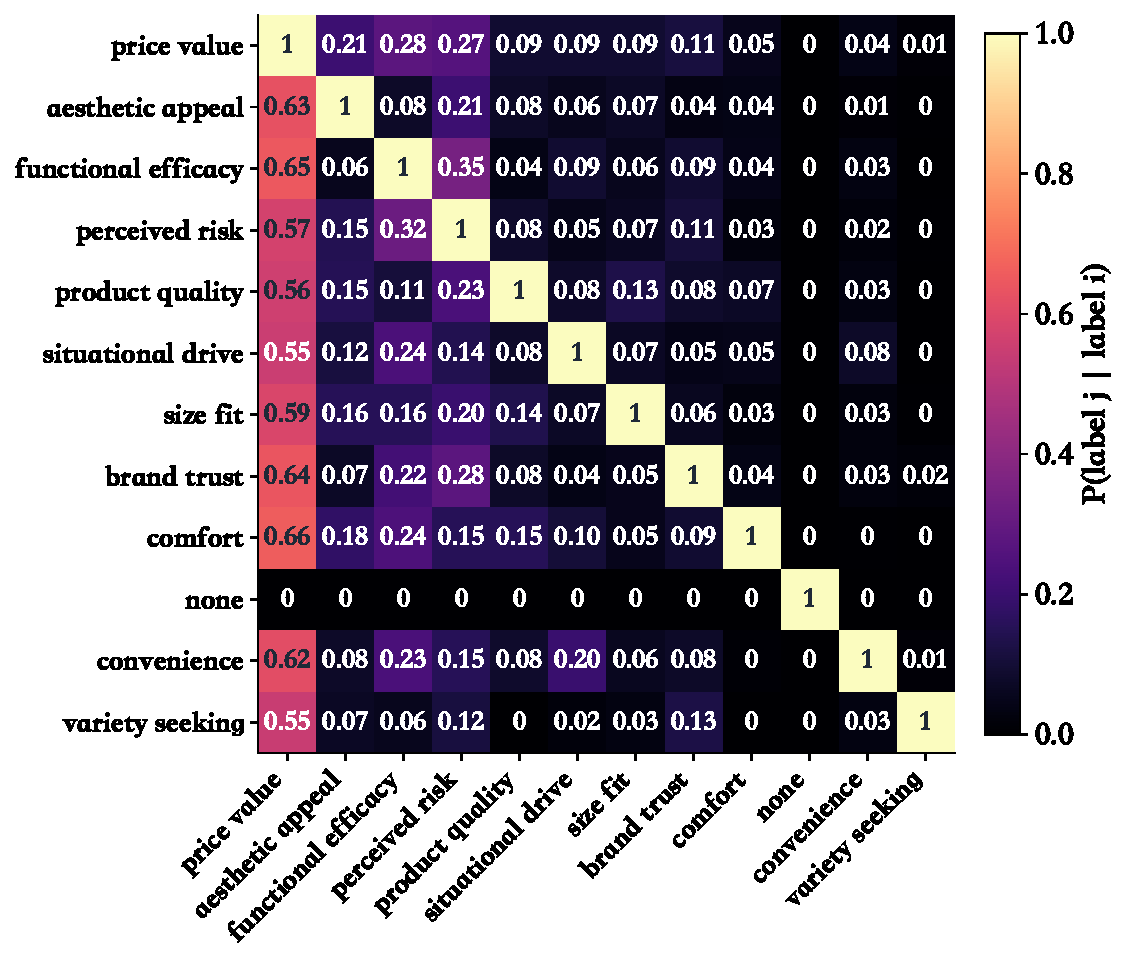
\includegraphics[width=\linewidth]{image/figs/fig7_cooccurrence.pdf}
  \caption{Label co-occurrence ratio}
  \label{fig:b2v:cooccur}
\end{subfigure}\hfill
\begin{subfigure}{0.32\textwidth}
  \centering
  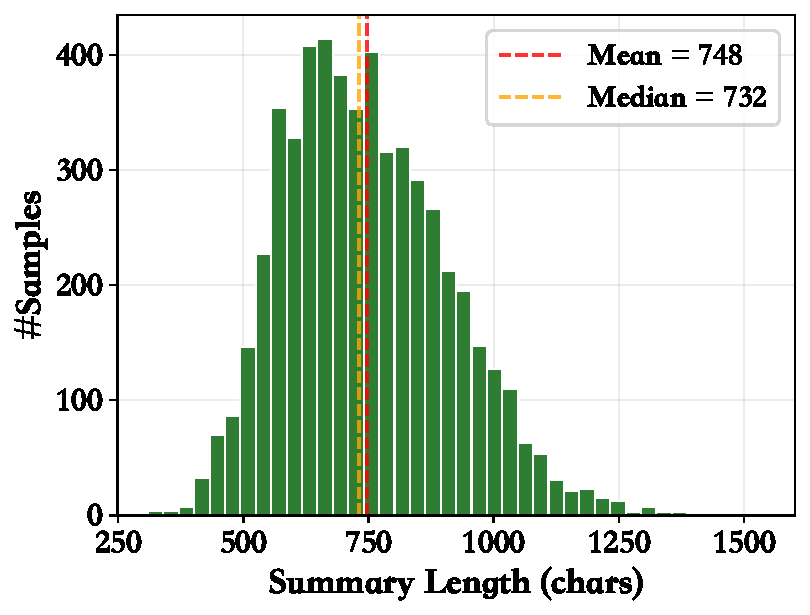
\includegraphics[width=\linewidth]{image/figs/fig3_length_hist.pdf}
  \caption{Summary length distribution}
  \label{fig:b2v:len}
\end{subfigure}

\vspace{6pt}

\begin{subfigure}{0.32\textwidth}
  \centering
  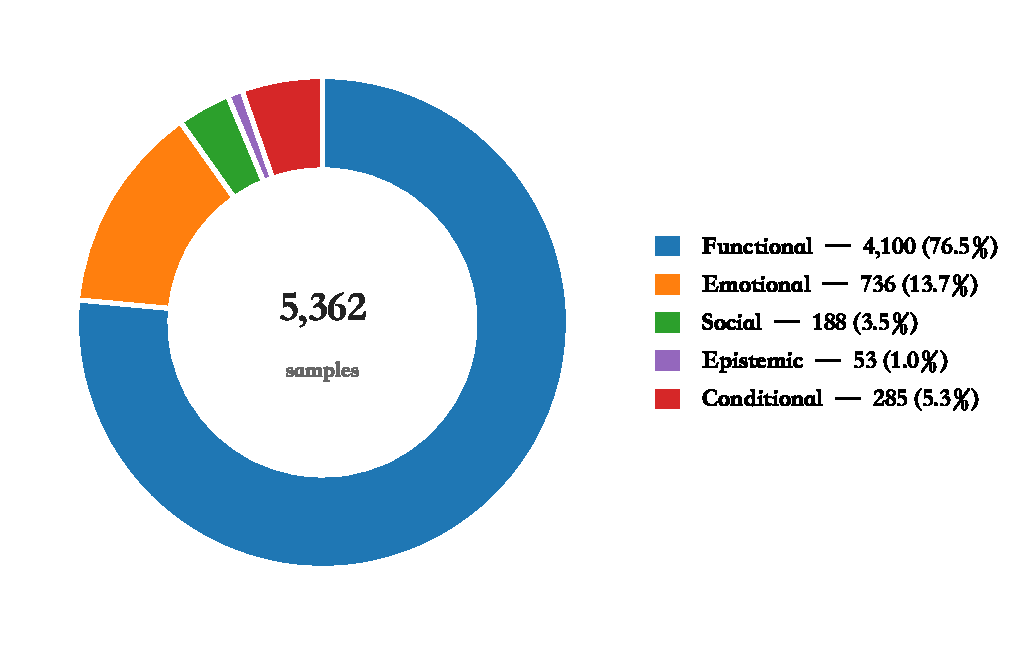
\includegraphics[width=\linewidth]{image/figs/fig5_tcv_pie.pdf}
  \caption{TCV dimension composition}
  \label{fig:b2v:tcv}
\end{subfigure}\hfill
\begin{subfigure}{0.32\textwidth}
  \centering
  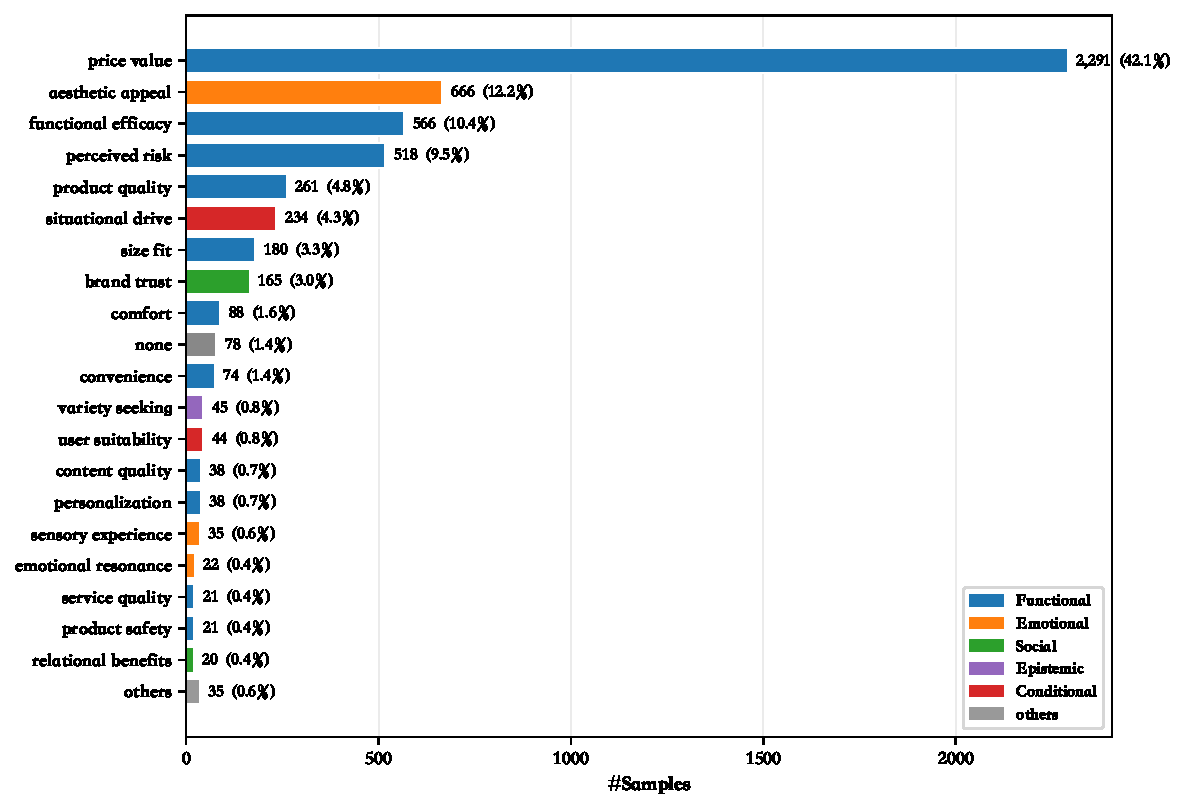
\includegraphics[width=\linewidth]{image/figs/fig4_label_bar.pdf}
  \caption{Per-label sample distribution}
  \label{fig:b2v:labelbar}
\end{subfigure}\hfill
\begin{subfigure}{0.32\textwidth}
  \centering
  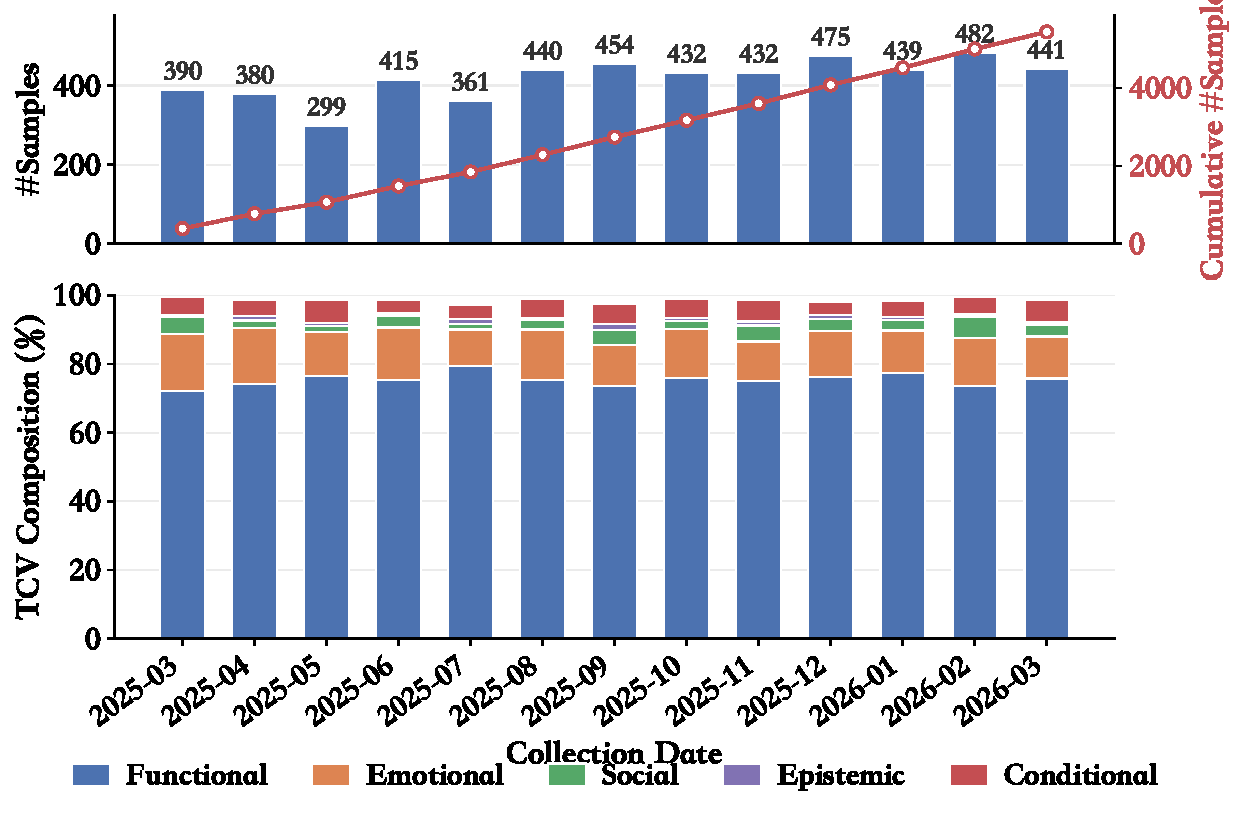
\includegraphics[width=\linewidth]{image/figs/fig6_per_date_stacked.pdf}
  \caption{Temporal coverage by TCV}
  \label{fig:b2v:time}
\end{subfigure}
\caption{Data analysis on \emph{B2V}.
(a) and (e) illustrate the long-tail label distribution
(Zipf slope $-2.25$; \emph{price~value} alone covers 42.1\% of samples);
(b) reports the conditional co-occurrence ratio
$P(\text{label}_j\mid\text{label}_i)$ among the 12 most frequent labels;
(c) shows the per-session summary-length distribution (mean 748, median 732
characters);
(d) maps the 30 value constructs onto the five TCV dimensions;
(f) shows that the dataset spans 13 monthly snapshots with stable TCV
composition over time.}
\label{fig:b2v-overview}
\end{figure*}

\subsection{Label Frequency, Imbalance and Co-occurrence}
The empirical label distribution of B2V follows a heavily skewed long tail.
Figure~\ref{fig:b2v:labelbar} lists the 28 distinct primary labels actually
used by human annotators: \emph{price~value} alone covers 42.1\% of the
samples, the top-5 labels account for 79\%, and the bottom 10 labels each
appear in fewer than 1\% of sessions. On a log-log scale
(Figure~\ref{fig:b2v:zipf}) the rank--frequency relation admits a near-linear
fit with slope $-2.25$, indicating a Zipf-like decay even steeper than the
standard $\alpha\!\approx\!1$; the corresponding Gini coefficient of the
label mass is $0.77$. Because of this imbalance, we report not only Accuracy
but also macro-averaged F1 in Section~\ref{sec:benchmark}, so that rare
constructs receive equal weight in evaluation.

Beyond marginal frequency, 75.2\% of sessions carry at least one secondary
value beyond the primary label, supporting evaluation under both single-label
and multi-label formulations. Figure~\ref{fig:b2v:cooccur} reports the
conditional co-occurrence matrix among the 12 most frequent labels, where
cell $(i,j)$ is
$P(\text{label}_j \in \text{sample} \mid \text{label}_i \in \text{sample})$.
Two patterns stand out. First, \emph{price~value} appears as a near-universal
co-driver: conditioned on almost any other label, the probability of
\emph{price~value} also being mentioned exceeds 0.55. Second, several pairs
exhibit strong directional asymmetries (e.g., \emph{functional efficacy}
$\to$ \emph{perceived risk} $=0.35$, \emph{brand~trust}
$\to$ \emph{perceived risk} $=0.28$), which motivates the 15 if--then
disambiguation rules used during annotation and model prompting.

\subsection{TCV Composition and Session Length}
Mapping the 30 constructs onto the five dimensions of the Theory of
Consumption Values (Functional, Emotional, Social, Epistemic, Conditional)
yields the composition in Figure~\ref{fig:b2v:tcv}: Functional values
dominate at 76.5\%, followed by Emotional (13.7\%), Conditional (5.3\%),
Social (3.5\%) and Epistemic (1.0\%). This is consistent with the broader
pre-purchase nature of the sessions in B2V, where instrumental concerns such
as price--value, functional efficacy and perceived risk drive most
decisions, while Epistemic and Social drivers appear less frequently but
more selectively. Per-sample summary length, shown in
Figure~\ref{fig:b2v:len}, is approximately log-normal: the mean is 748 and
the median 732 Chinese characters, with the bulk of sessions falling between
500 and 1000 characters. Emotional decisions are described at slightly
greater length than Social or Epistemic decisions (median 770 vs.\ ${\sim}660$
characters), suggesting that aesthetic and affective drivers tend to
manifest through longer chains of observable behavior.

\subsection{Temporal Coverage and Split Balance}
B2V is collected across 13 monthly snapshots spanning March 2025 to March
2026, totaling 5{,}440 annotated sessions and 202{,}771 extracted behavior
interactions. Figure~\ref{fig:b2v:time} shows the per-snapshot session
count together with the normalized composition of TCV dimensions over time.
Volumes range from 299 to 482 sessions per snapshot and the cumulative
collection grows monotonically. The TCV composition is stable across
snapshots: Functional values remain dominant throughout, while Emotional,
Conditional, Social and Epistemic shares stay within $\pm$3\% of their
global means. This indicates that the dataset captures consistent decision
behavior across a one-year window rather than reflecting a single seasonal
pattern.

We further adopt an 80/10/10 stratified split at the session level. Across
the 12 most frequent labels, the largest deviation between any split and
the corpus average is 2.9 percentage points (\emph{aesthetic~appeal} in
test, 14.7\% vs.\ 11.9\% overall); the remaining labels agree within
$\pm$2\%. Total token-level statistics in Table~\ref{tab:b2v-stats}
further confirm that average session length, behavior--interaction count
and TCV composition match closely across train, validation and test.


\section{Method}
Building on the Behavior2Value dataset, we propose B2V-Model, a behavior-to-value large language model obtained by applying Value Verification Tuning (VVT) to Qwen3-8B. Unlike standard supervised fine-tuning, which directly learns a mapping from behavior sequences to value labels, VVT formulates B2V as a value judgment verification problem. Given a user’s pre-purchase behavioral trajectory, the model is required not only to predict the consumption values that may be reflected in the behavior, but also to assess whether each value judgment is sufficiently supported by behavioral evidence.

Specifically, for each behavioral episode, we organize the information produced during annotation into structured supervision signals, including the accepted value labels, rejected candidate value labels, supporting evidence, counter-evidence, and boundary rules that distinguish between value constructs. The model is trained to first identify key evidence from the behavioral sequence, then verify candidate value judgments according to value definitions and construct-level boundaries, and finally output the evidence-supported value labels together with their explanations. In this way, VVT uses not only positive labels to supervise what the model should predict, but also rejected labels and counter-evidence as hard negatives, guiding the model to learn which seemingly relevant value judgments should not be accepted.

This verification-oriented training paradigm better aligns with the nature of the B2V task. Consumption values are not directly observable categories, but latent constructs that must be inferred from indirect, sparse, and often ambiguous behavioral evidence. As a result, classification-based SFT can easily learn shortcut associations between surface behaviors and value labels, leading to excessive or unsupported value attribution. In contrast, VVT explicitly models the validity conditions of value judgments, enabling the model to learn how to accept, reject, and distinguish value judgments based on evidence. This improves its ability to discriminate between closely related value constructs and produces explanations that are more faithful and auditable.




\section{Benchmarking the Behavior-to-Value Task}

\section*{Limitations}




% Bibliography entries for the entire Anthology, followed by custom entries
%\bibliography{custom,anthology-overleaf-1,anthology-overleaf-2}

% Custom bibliography entries only
\bibliography{custom}

\appendix

\section{Example Appendix}
\label{sec:appendix}

This is an appendix.

\end{document}
